\chapter{Durchführung}
\label{cha:Durchführung}
Um ein Verständnis für den Laser, sowie das Verhalten bei verschiedenen Parametern zu erarbeiten werden verschiedene Messungen durchgeführt. Dafür wird zunächst der Laser mit den 
Steuer- und Messelementen verkabelt.

\section{Bestimmung des Schwellenstroms}
\label{sec:schwelle}

Um den Schwellenstrom zu messen, ab welchem der Laserbetrieb gewährleistet ist, wird der erwartete Laserstrahl mit einer Detektorkarte untersucht. Diese Detektorkarte reflektiert 
Infrarot so, dass es im optischen Bereich liegt. Mit einer CCD Kamera kann die Reflexion aufgenommen werden. Wird nun der Diodenstrom erhöht, tritt ab einem Schwellenwert
ein selbstverstärkender Effekt auf. Zusätzlich lässt sich ein charakteristisches fleckiges geflecktes Muster auf der Karte beobachten. Dies geschieht aufgrund von Beugungseffekten an einer unebenen Oberfläche.
Sobald dieses Muster auftritt und die Intensität deutlich ansteigt ist der Schwellenstrom erreicht. Dieser wird notiert.

\section{Aufnahme der Rubidiumfluoreszenz}
\label{sec:fluoreszenz}

Als nächstes wird der aktive Laser auf eine Rubidiumzelle gerichtet. Diese ist mit einem Rubidium-Gasgemisch gefüllt, welches aus Rb-85 und Rb-87 besteht. Durch Relaxationsprozesse kann Fluoreszenz mit einer CCD Kamera aufgenommen werden. Wie in Abschnitt \ref{sec:rub}
beschrieben, tritt dies allerdings nur für exakt definierte Wellenlängen auf. Die Wellenlänge kann durch Drehung des Gitters, und somit der Veränderung der Länge des äußeren Hohlleiters, variiert werden. Dies geschieht, bis man Fluoreszenz beobachtet.

\section{Absorptionsspektrum von Rubidium}
\label{sec:abso_rub}

Um das Absorptionsspektrum von Rubidium zu messen wird ein Versuchaufbau nach Abbildung \ref{fig:Aufbau_rub} gebaut.

\begin{figure}
    \centering
    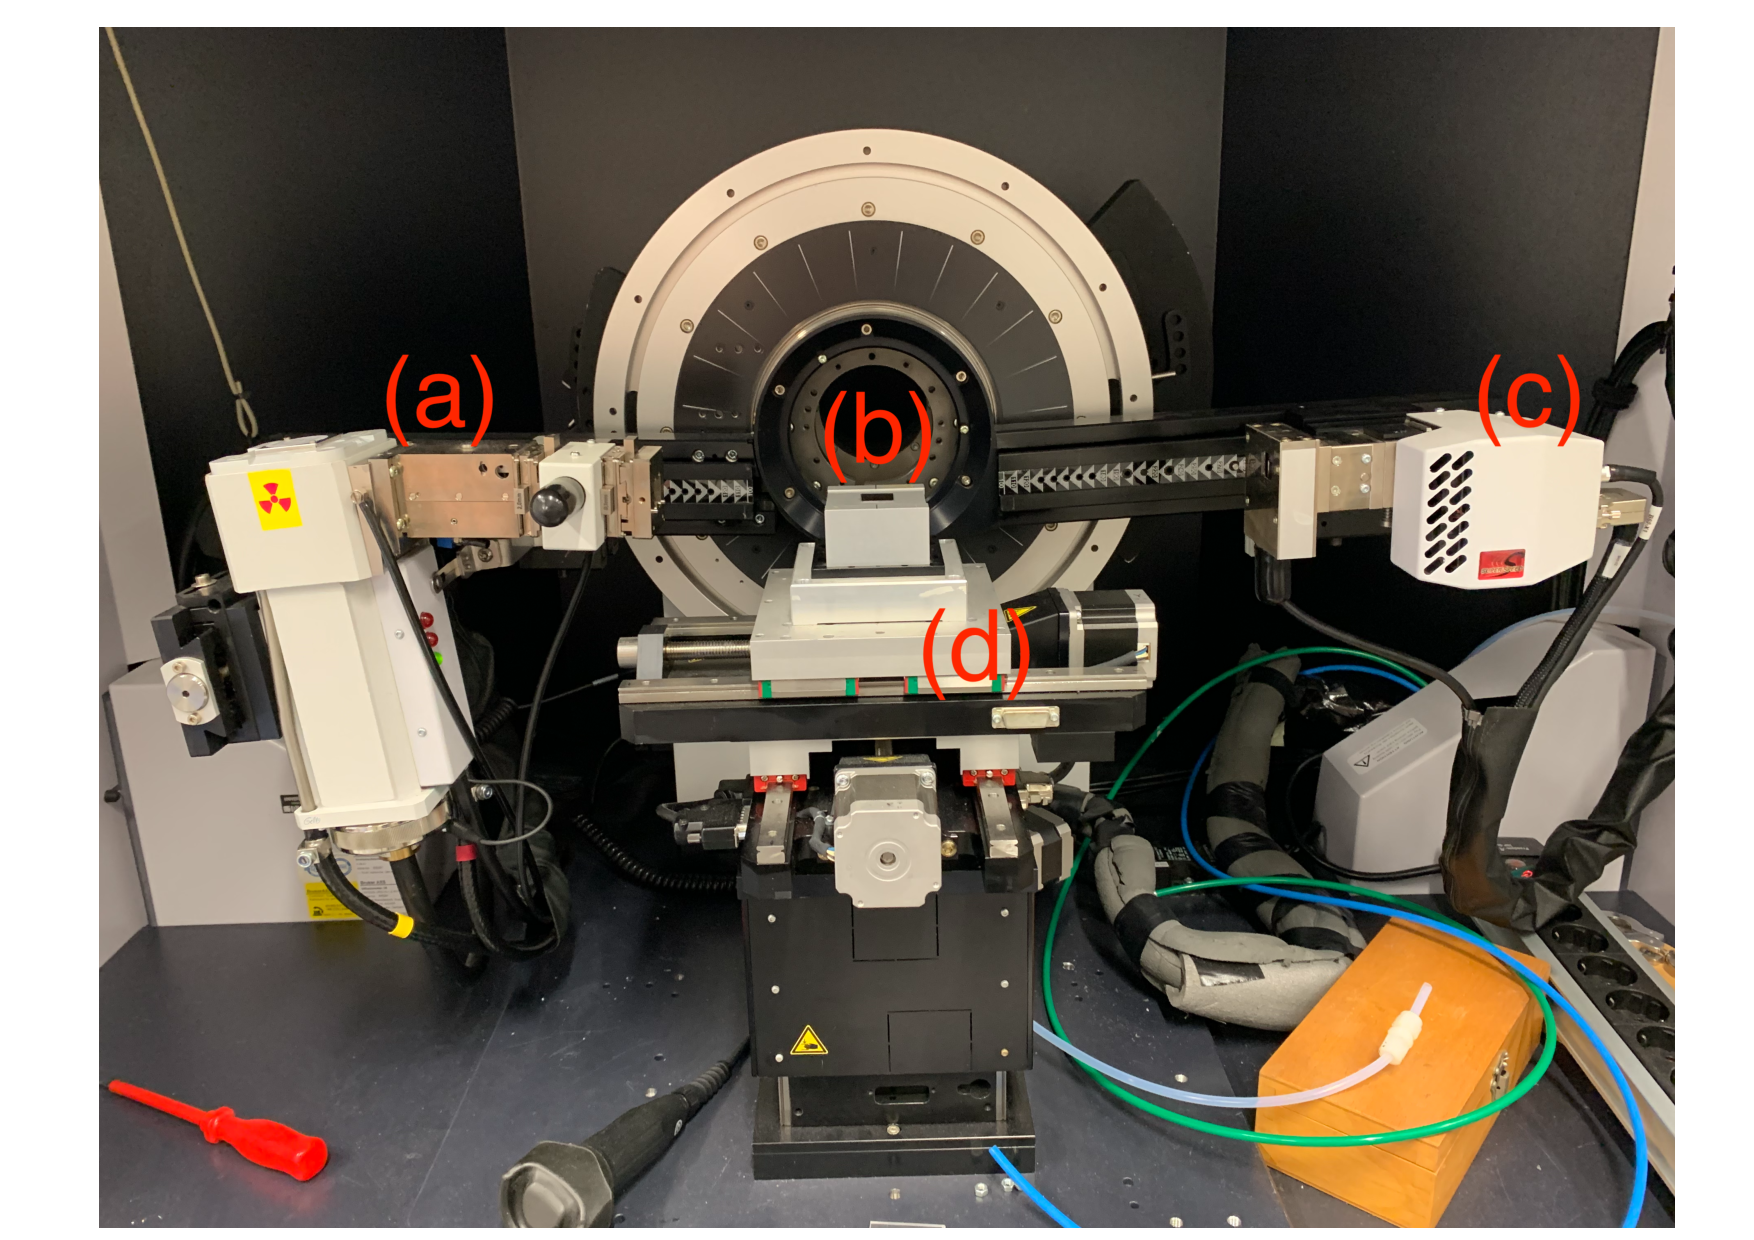
\includegraphics[width=\textwidth]{bilder/Aufbau.png}
    \caption{Verwendeter Versuchsaufbau zur Bestimmung des Absorptionsspektrums der Rubidiumzelle \cite{diode_laser_spectroscopy}.}
    \label{fig:Aufbau_rub}
\end{figure}

Der Laser trifft zunächst auf einen 50/50 Strahlteiler. Ein Teil des Strahls wird direkt in eine Photodiode eingespeist und der andere Teil wird durch die Rubidiumzelle auf eine
weitere Photodiode gestrahlt. Mithilfe eines Oszilloskops kann schließlich das Differenzsignal dargestellt werden. Dies ist notwendig, um Hintergrundrauschen zu minimieren und ein möglichst 
genaues Spektrum zu erhalten. Der Strom wird gemäß einer Dreiecksschwingung linear um einen Nullwert erhöht und gesenkt, um das Absorptionsspektrum des Rubidiumgases in Abhängigkeit
der Wellenlänge darstellen zu können.
